%% ACM Transactions on Storage submission -- v2, evidence-constrained rewrite
%% following the pre-submission audit. Review format per current ACM journal
%% guidance: single column, line numbers via `review`.
\documentclass[manuscript,screen,review]{acmart}

\usepackage{booktabs}
\usepackage{graphicx}

\begin{document}
% generated by sweep/prose_numbers.py -- do not edit
\newcommand{\pFoldWriteBlock}{60}
\newcommand{\pFoldWriteFile}{27}
\newcommand{\pFoldWriteObject}{1.0}
\newcommand{\pFoldReadBlock}{54}
\newcommand{\pFoldReadFile}{51}
\newcommand{\pFoldReadObject}{1.2}
\newcommand{\consCellsTotal}{30}
\newcommand{\consCellsWithin}{28}
\newcommand{\consGeoMean}{1.08}
\newcommand{\azureVOneWriteBeta}{0.001}
\newcommand{\azureVTwoWriteBeta}{0.310}
\newcommand{\azureWriteRatio}{2.36}
\newcommand{\designFixed}{174}
\newcommand{\designScaled}{162}
\newcommand{\designOther}{24}
\newcommand{\gatedRuns}{71}
\newcommand{\gatedPct}{19.7}



\title{Concurrency Scaling of Managed Cloud Storage: A Retrospective
Measurement Study of Block, File and Object Paradigms on Five Public Clouds}

\author{Tshivhidzo Makungo}
\email{makungotshivhidzo@gmail.com}
\affiliation{%
  \institution{Cape Peninsula University of Technology}
  \city{Cape Town}\country{South Africa}}
\author{Boniface Kabaso}
\email{kabasob@cput.ac.za}
\affiliation{%
  \institution{Cape Peninsula University of Technology}
  \city{Cape Town}\country{South Africa}}

\begin{abstract}
Selection guidance for managed cloud storage compares block, file and object
services at fixed client parallelism; how delivered performance changes as
offered concurrency rises is largely uncharacterised across providers. We
report a 360-run measurement campaign on five public clouds (AWS, Microsoft
Azure, Google Cloud, Huawei Cloud, Alibaba Cloud) measuring three managed
storage paradigms under two data-movement workload classes at 1, 4, 16 and 64
client threads with three repetitions per cell. Per-operation throughput
(write-phase and read-phase rates, and a combined rate computed as total bytes
over total elapsed time) is summarised as a fitted power-law exponent $\beta$
with a 95\% confidence interval. All 30 provider--paradigm--workload cells
reached full concurrency coverage; final coverage required 611 attempts for
360 accepted runs, and all attempts are archived. Because instrument
corrections were applied during the campaign, executed conditions vary in
documented ways (dataset sizing rule, phase time limits, one runner version,
one endpoint change); we therefore present this as a retrospective study with
a complete as-executed audit, and we publish a locked protocol for a planned
replication. Findings: object storage scaled near-linearly for small-operation
traffic on four of five clouds ($\beta$ 0.85--1.00, $R^2 \geq 0.97$); Azure
Blob is the exception ($\beta = 0.36$). Block storage at entry tiers showed no
useful scaling on any cloud (combined-rate $\beta \leq 0.11$, and $\leq 0.10$
on four of five), and file storage was intermediate (0.18--0.69). Tail
latency moved oppositely: from 1 to 64 threads, median write-phase p99 grew
\pFoldWriteBlock-fold on block and \pFoldWriteFile-fold on file but was flat on scaling object stores. A
mixed-effects test with paradigm and workload fixed effects, over the 356
runs with a defined paired-pass rate, found no evidence of
provider-dependent scaling slopes (LR $= 0.44$; boundary-corrected
$p = 0.65$; parametric bootstrap $p = 0.55$ over 200 valid draws under an
explicit finite-likelihood and nested-ordering validity policy, with
per-draw records archived), within the power limits of five provider
groups. We also document two instrument defects
whose signatures could be mistaken for service behaviour: a client-runner
concurrency defect and an endpoint-path bandwidth cap. All raw artefacts,
including quarantined defective-instrument data, are openly archived.
\end{abstract}

\begin{CCSXML}
<ccs2012>
<concept>
<concept_id>10002951.10003152.10003517</concept_id>
<concept_desc>Information systems~Cloud based storage</concept_desc>
<concept_significance>500</concept_significance>
</concept>
</ccs2012>
\end{CCSXML}
\ccsdesc[500]{Information systems~Cloud based storage}

\keywords{cloud storage, benchmarking, concurrency, scalability, measurement
study, object storage, block storage, file storage}

\maketitle

\section{Introduction}
Public clouds offer three managed storage paradigms with different
architectures: block volumes attached to virtual machines, file shares served
over NFS or SMB, and object stores addressed through HTTP APIs. Published
comparisons, including our own earlier work \cite{thesis}, measure these
paradigms at one level of client parallelism. Provisioning decisions, however,
depend on a different question: what happens to delivered performance when an
application raises its offered concurrency?

The paradigms suggest different answers. An object store distributes requests
over a horizontally scaled service and might absorb added client parallelism
with little loss. A block volume is a provisioned resource whose tier defines
a throughput and IOPS envelope that additional threads must share. File
services add a protocol layer whose request discipline limits how much
parallelism converts into throughput. These expectations are widely held but
have not been quantified side by side across providers under one method.

This paper reports such a measurement. We extended the benchmark harness of
our fixed-concurrency study \cite{thesis} into a concurrency sweep: five
providers, three paradigms, two data-movement workload classes, four
concurrency levels (1, 4, 16, 64 threads), three repetitions, 360 designed
runs. Behaviour per cell is summarised by a fitted exponent $\beta$
(throughput $\propto$ concurrency$^{\beta}$).

Two aspects of how we report this work need stating plainly at the outset.
First, final coverage is complete -- each of the 360 designed runs produced
an accepted measurement -- but completeness was reached through documented
retries: 611 attempts in total, dominated by one provider's object-storage
control-plane interactions (Table~\ref{tab:attempts}). Every attempt, failed
or accepted, is preserved in append-only manifests in the public archive.
Second, the campaign doubled as the shakedown of its own instrument. Four
corrections were applied while it ran (dataset sizing rule, phase time limits,
one runner replacement, one endpoint change), so executed conditions are not
uniform across the dataset. Section~\ref{sec:asexecuted} quantifies exactly
which runs executed under which conditions, the analysis in
Section~\ref{sec:results} uses only quantities that are well-defined for
every run, and a locked protocol for a uniform replication is published with
the archive. We present the study as a retrospective analysis under those
disclosures rather than as the execution of a single design fixed and
independently registered in advance; no analysis choice in this paper has
an independent timestamped registration predating data collection, and we
label the statistics exploratory accordingly.

The contributions are: (1) a public 360-run dataset of concurrency-scaling
measurements for managed storage on five clouds, with raw tool output,
telemetry, manifests recording every attempt, and quarantined
defective-instrument data preserved for audit; (2) per-operation scaling
exponents with confidence intervals for all cells, computed by an archived
pipeline directly from raw artefacts, with client-CPU sensitivity refits;
(3) a per-phase tail-latency characterisation; (4) an as-executed design
audit that quantifies the campaign's non-uniformities instead of asserting
uniformity; and (5) two documented instrument failure modes -- a client
runner whose concurrency defect produced curves resembling service
saturation, and an endpoint choice that silently measured a gateway
bandwidth cap -- with the evidence archived.

\section{Related Work}
Cross-provider cloud measurement began with CloudCmp \cite{cloudcmp}; YCSB
\cite{ycsb} standardised workload classes for cloud serving systems; Schad et
al.\ \cite{schad} established the variance discipline that motivates our
repetitions and disclosure rules; Iosup et al.\ \cite{iosup} and Uta et
al.\ \cite{uta} developed the case for repeated, archived cloud performance
measurement. Storage benchmarking methodology has its own critical tradition:
Traeger et al.'s survey of file system and storage benchmarking practice
\cite{traeger} catalogues the reporting failures -- unstated configurations,
unnamed bottlenecks, unrepeatable setups -- that our archive-first design is
built to avoid. COSBench \cite{cosbench} established configurable object-store
benchmarking; Hou et al.\ characterised cloud object-storage I/O
behaviour from the client's perspective on a single provider class,
the closest antecedent to our client-side method \cite{hou}; CNSBench \cite{cnsbench} addressed cloud-native storage; Durner
et al.\ \cite{durner} characterised object-store request parallelism on a
single provider class; Leis and Kuschewski \cite{leis} model storage bandwidth
in cloud query cost; Anna \cite{anna} shows what a storage tier designed for
elasticity achieves. General benchmarking methodology is treated by Bermbach
et al.\ \cite{bermbach}. We are not aware of published concurrency-scaling
exponents for the three managed paradigms measured side by side across five
public clouds; that is the specific gap addressed here.

The exponent framing follows the parallel-systems tradition of Amdahl
\cite{amdahl}, Gustafson \cite{gustafson} and Gunther \cite{gunther}: a
log--log slope over a thread sweep is the minimal empirical summary that is
comparable across services and makes no mechanistic assumption.

\section{Method}
\subsection{Harness and Integrity Rules}
For every run the harness provisions the storage target afresh via Terraform,
drops caches, warms up 60 seconds, measures, records guest CPU telemetry
(\texttt{mpstat}, 5-second cadence), stores the tool's raw output verbatim
with a SHA-256 digest, and tears the target down. An append-only manifest
records every attempt with its full command line (credential values masked).
Failed attempts produce no metrics and are never imputed. Block and file runs,
and object runs on the four S3-compatible clouds, use elbencho 3.1-1
\cite{elbencho}; Azure Blob object runs use a purpose-built SDK runner
(Section~\ref{sec:instrument}).

\subsection{Design and As-Executed Conditions}\label{sec:asexecuted}
The design grid is 5 providers $\times$ 3 paradigms $\times$ 2 workload
classes $\times$ 4 concurrency levels $\times$ 3 repetitions. Benchmark hosts
are one 4 vCPU / 16 GB instance per provider, co-located with storage targets
(regions and SKUs in Table~\ref{tab:config}). The \emph{balanced} class moves
64 KiB operations in a write pass then a read pass, equal volume; the
\emph{large-object} class streams 16 MiB objects, a preparation write
(unmeasured) followed by a measured sequential read. No interleaved
read/write mixing and no random-access pattern is present in either class.

Because corrections were applied mid-campaign, executed conditions vary, and
we report them from the archived command lines rather than from the design
intent. Dataset sizing: \designFixed{} runs executed with fixed totals (20 GB balanced,
40 GB large-object at every level), \designScaled{} with weak scaling (base $\times$
concurrency/16, capped at 80 GB), and \designOther{} Azure object runs are duration-driven
(no dataset target); 12 of 120 provider-cells mix sizing rules across
repetitions. Under the capped weak-scaling rule the large-object c64 cells run
at half the constant per-thread allocation, so even the weak-scaled subset is
not uniform weak scaling at the top level. Phase time limits: 35 of the 240
accepted block/file runs carry \texttt{--timelimit 600}; a consequence of elbencho's
semantics (the limit ends the whole benchmark, not the phase) is that four
Azure block balanced runs measured a write phase only, and they are flagged
as such in the dataset. All Alibaba object results use the region-internal
endpoint; runs recorded against the public endpoint are excluded and
quarantined (Section~\ref{sec:instrument}). These non-uniformities motivate
two analysis decisions: throughput is analysed per operation at steady state
(rates are well-defined regardless of dataset size or truncation), and every
run's conditions ship with the dataset so any alternative slicing can be
recomputed. A locked protocol (uniform 20 GB base for both classes, reaching
the 80 GB ceiling exactly at c64; universal time limits; pinned instrument
hashes; fixed retry rule) is published in the archive for replication.

\begin{table}
\caption{Attempts versus accepted runs per provider. Failures are dominated
by provisioning-level interactions (object-store bucket lifecycle on Alibaba;
endpoint and runner corrections on Azure and GCP), not by measurement
variability. All attempts are preserved in the archived manifests. Retry rule
as executed: failed runs were re-attempted until accepted or until the
underlying defect was diagnosed and corrected; the locked replication
protocol fixes a maximum of two retries.}
\label{tab:attempts}
\begin{tabular}{lrr}
\toprule
Provider & Attempts & Accepted \\
\midrule
AWS & 85 & 72 \\
Azure & 114 & 72 \\
GCP & 104 & 72 \\
Huawei & 81 & 72 \\
Alibaba & 227 & 72 \\
\midrule
Total & 611 & 360 \\
\bottomrule
\end{tabular}

\end{table}

\begin{table}
\caption{As-executed configuration summary (full table with sources and
unrecoverable items marked is in the archive: configs/AS\_EXECUTED\_CONFIG.md).
NIC limits are provider-documented figures for the SKU, not measurements; the
replication protocol adds a measured per-host network baseline.}
\label{tab:config}
\resizebox{\textwidth}{!}{%
\begin{tabular}{llllll}
\toprule
 & AWS & Azure & GCP & Huawei & Alibaba \\
\midrule
Region & af-south-1 & southafricanorth & africa-south1 & af-south-1 & me-central-1 \\
Host SKU & m5.xlarge & D4s\_v3 & e2-standard-4 & c6.xlarge.4 & ecs.hfg6.xlarge \\
Block & gp3, 100 GB & StdSSD LRS, 100 GB & pd-ssd, 100 GB & EVS SSD, 100 GB & cloud disk, 100 GB \\
File & EFS GP, elastic (no fixed size) & Files Std (SMB), 100 GB quota & Filestore BASIC\_HDD, 1{,}024 GB & SFS Turbo, 500 GB & NAS Capacity (NFS), pay-per-use \\
Object & S3 Std & Blob StdV2 LRS & GCS Std & OBS Std & OSS Std (internal ep.) \\
\bottomrule
\end{tabular}}
\end{table}

\subsection{Metrics and Analysis}\label{sec:metrics}
{\sloppy All reported numbers are recomputed from raw artefacts by an
archived pipeline (\texttt{sweep/recompute\_from\_raw.py},
\texttt{sweep/refit\_exponents.py}, \texttt{sweep/make\_figures.py},
\texttt{sweep/prose\_numbers.py}); the principal exponent tables, the attempt table and the specified prose
statistics are generated directly by the archived pipeline
(\texttt{table\_combined}, \texttt{table\_perop},
\texttt{table\_attempts}, \texttt{prose\_macros.tex}); remaining reported
values are traceable to its outputs or to the archived configuration
records.\par} Per run we compute: write-phase throughput and read-phase throughput,
each as the phase's total MiB divided by the phase's elapsed seconds from the
tool's own totals; a combined rate defined as total MiB of both phases over
total elapsed seconds of both phases (reported only for runs with both
phases); and per-phase p99 latency from the tool's per-phase percentile
output. Sequential phase rates are never summed, and percentiles are never
combined across phases. For elbencho csv files, which append across retry
attempts, the final attempt's phase rows are selected deterministically (the
stdout log, overwritten per attempt, is inherently final).

Exponents: OLS of $\log_{10}$(metric) on $\log_{10}$(concurrency) per
provider--paradigm--workload--operation, with $t$-based 95\% CIs. Sensitivity:
identical fits excluding runs whose mean client CPU exceeded 80\% (\gatedRuns{} runs,
\gatedPct\%). Pooled model: $\log_{10}$(combined) on $\log_{10}$(concurrency)
crossed with paradigm and workload as fixed effects, provider as a random
intercept; the provider random slope on log concurrency is tested against the
50:50 $\chi^2_1$:$\chi^2_2$ mixture appropriate to a boundary variance
component, and additionally by parametric bootstrap of the likelihood-ratio
statistic under the null. With five provider groups this test has limited
power, which the interpretation respects.

\subsection{Instrument Corrections and Quarantined Data}\label{sec:instrument}
Two instrument defects were found and corrected during the campaign. Both
defective datasets are preserved in the archive under \texttt{quarantine/}
with digests, so the corrections are auditable rather than asserted.

\emph{Azure Blob runner.} Azure Blob is not S3-compatible, so object runs use
an SDK-based runner. Its first version submitted work in synchronised batches
from one Python process; batch barriers plus interpreter-lock serialisation
of TLS work produced a throughput curve that rose to 4 threads and fell
thereafter -- a shape indistinguishable from service saturation. The
corrected runner (bounded process pool, independent deadline-driven loops,
socket timeouts, streaming reads, per-phase output) changes both the level
and the shape of the measurement. The like-for-like comparison is between
write phases, the only operation the defective runner actually performed:
the v1 write-only exponent is \azureVOneWriteBeta{} (flat), the corrected runner's
write-phase exponent is \azureVTwoWriteBeta, and the 16-thread write-to-write ratio is
\azureWriteRatio$\times$ (Figure~\ref{fig:azure} shows the qualitative shape contrast;
the two runners' full metrics are constructed differently and are not
compared numerically). All Azure object results in the dataset come from
the corrected runner; the defective runner's complete output is quarantined.
We note a reporting limitation: the deployed runner file's hash was not
recorded per run in this campaign (the runner version is identified by its
output schema and deployment record); the replication protocol records
per-run instrument hashes.

\begin{figure}
  \centering
  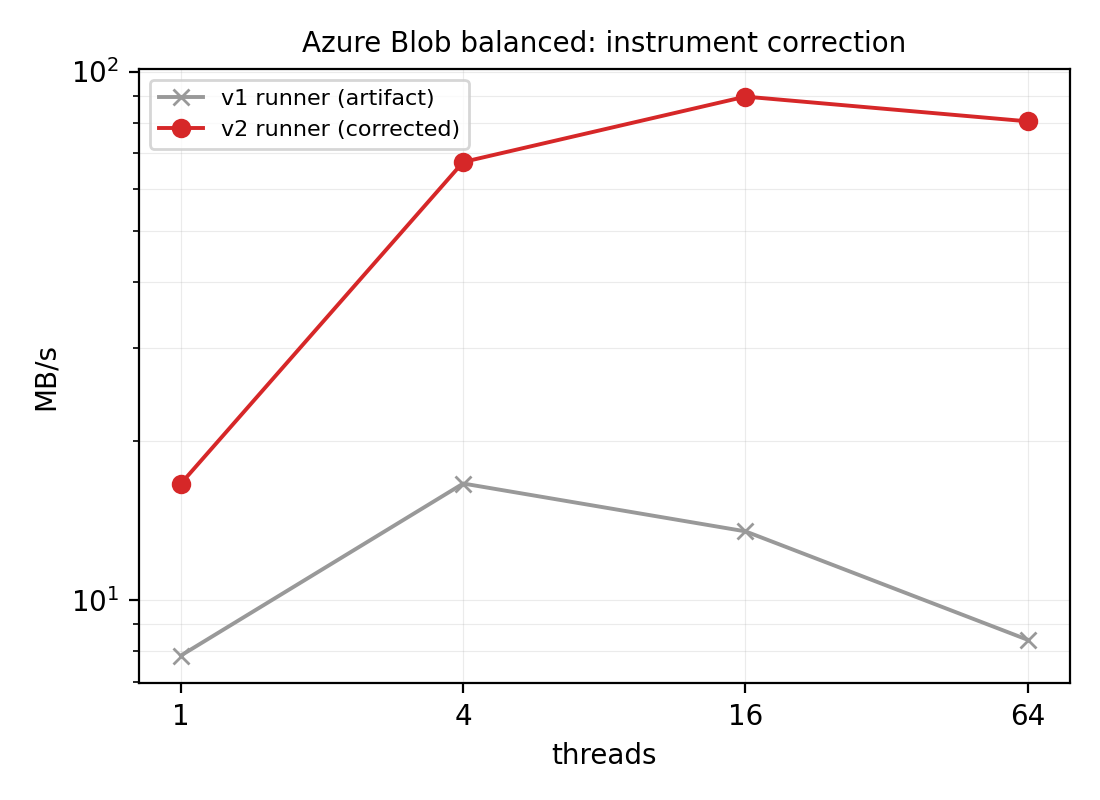
\includegraphics[width=0.6\columnwidth]{figures/fig3_azure_instrument}
  \caption{Azure Blob balanced throughput measured by the defective v1 runner
  (its own recorded single-phase rate) and the corrected v2 runner
  (paired-pass bytes over time). The v1 curve's rise-then-fall shape
  resembles service saturation but is a client concurrency defect; the two
  metrics are constructed differently, so shapes, not absolute ratios, carry
  the comparison. Both datasets are archived (v1 under
  \texttt{quarantine/}).}
  \Description{Line chart comparing two measurements of the same Azure Blob
  service: the defective runner's curve rises to four threads then falls,
  while the corrected runner's curve rises monotonically and saturates at
  sixteen threads at a much higher level.}
  \label{fig:azure}
\end{figure}

\emph{Alibaba endpoint.} Object traffic addressed to the region's public OSS
endpoint traverses the host's Internet gateway, whose bandwidth allowance
caps measured throughput. We measured the identical workload at 12 MiB/s via
the public endpoint and several hundred MiB/s via the region-internal
endpoint. Twelve runs accepted against the public endpoint were excluded and
quarantined; every object run's endpoint is part of its archived command
line.

\section{Results}\label{sec:results}
\subsection{Throughput Against Concurrency}
\begin{figure*}
  \centering
  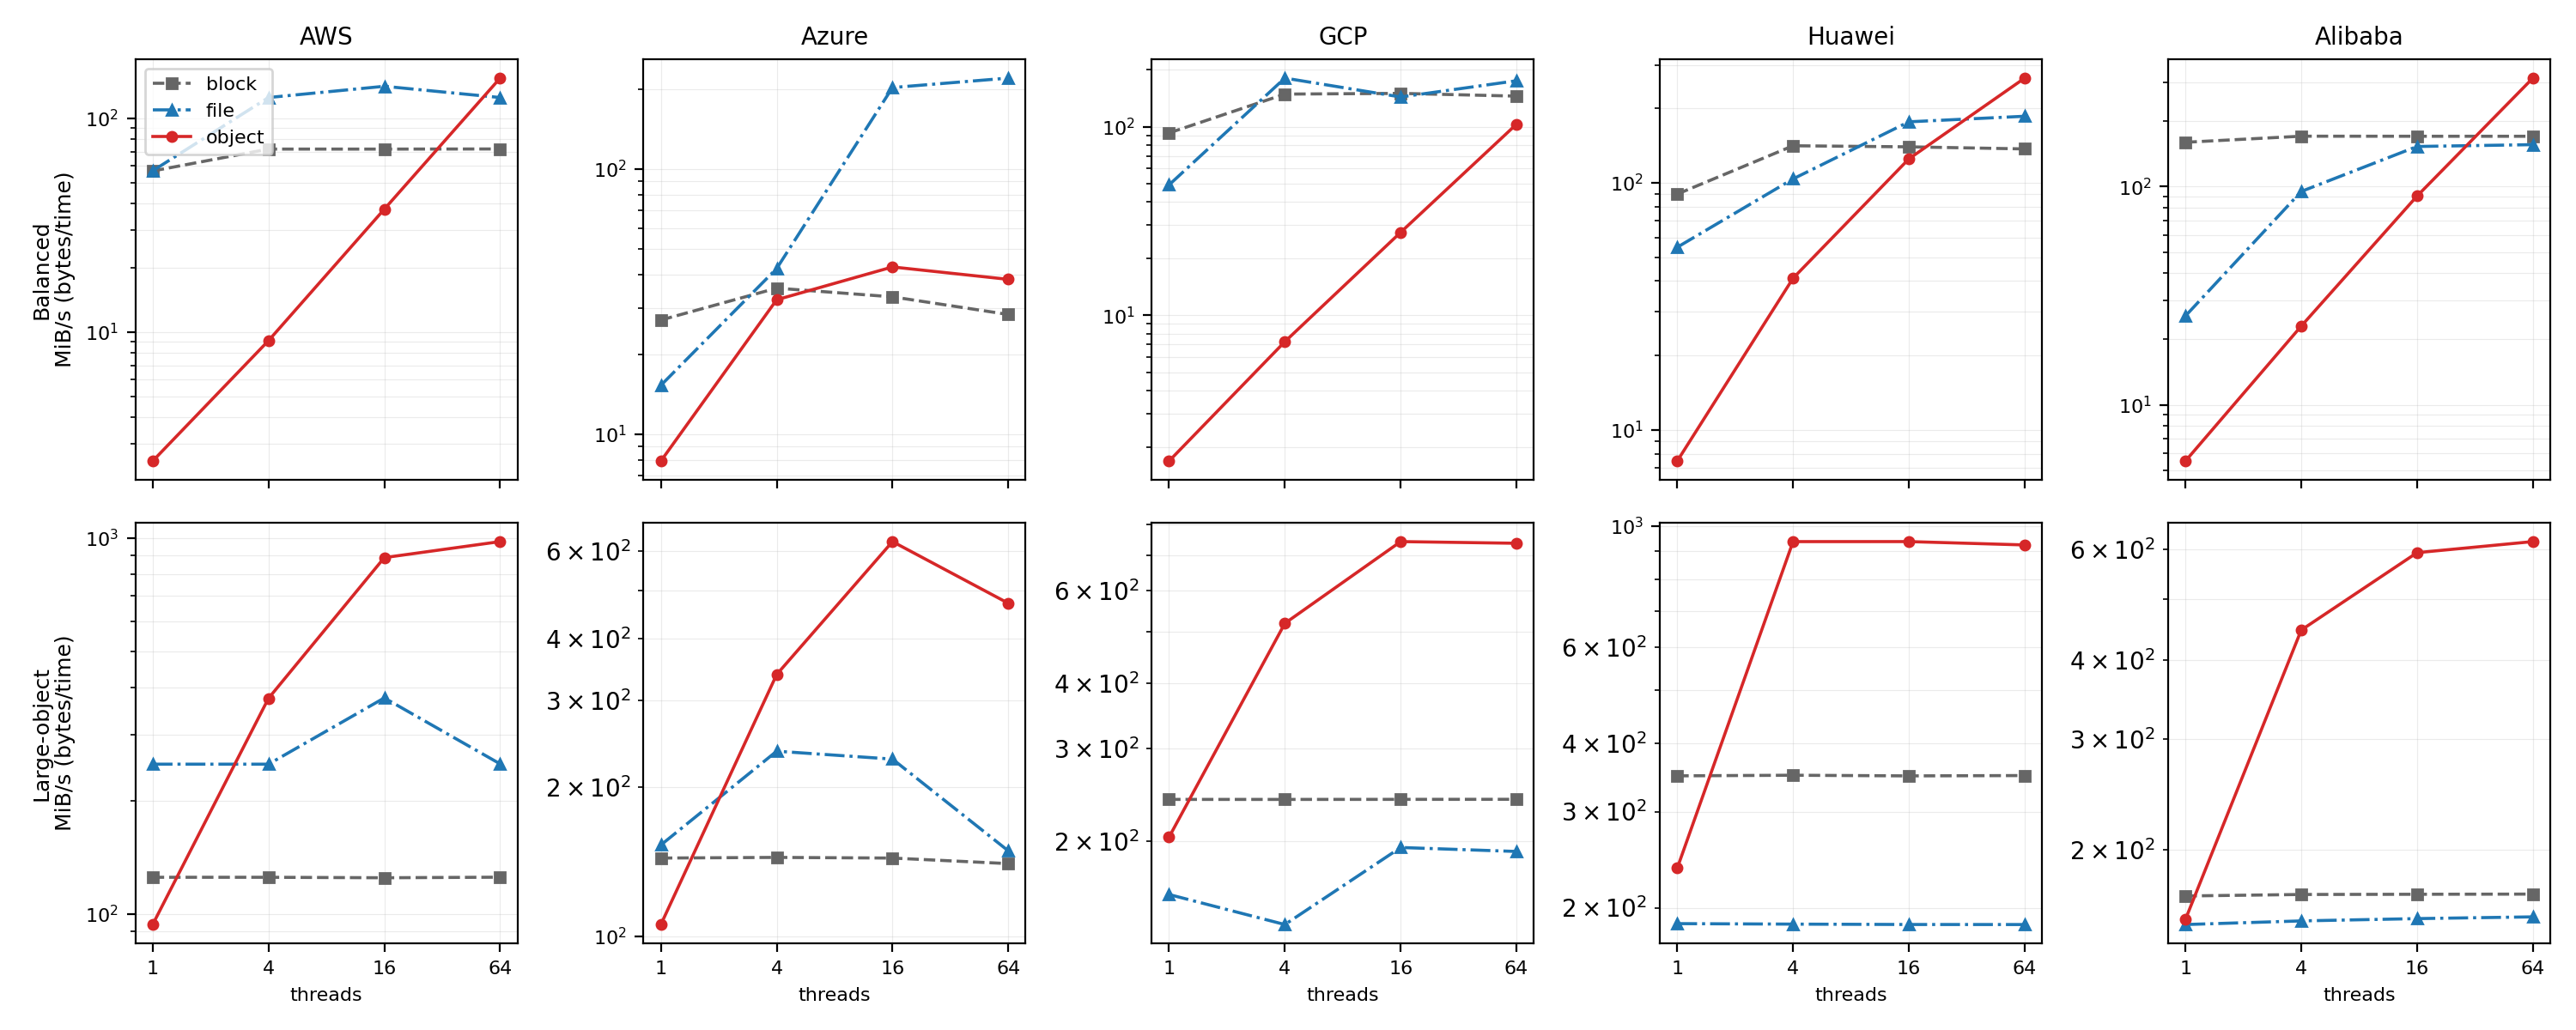
\includegraphics[width=\textwidth]{figures/fig1_recomputed}
  \caption{Combined throughput (total bytes over total elapsed time,
  log--log) against client threads for both workload classes on all five
  clouds. Cell means over three repetitions.}
  \Description{Ten log-log panels, one per cloud and workload class. Object
  storage lines rise steadily with thread count in the balanced class and
  flatten by sixteen threads in the large-object class; block storage lines
  are flat in both classes; file storage lines rise modestly then flatten.}
  \label{fig:curves}
\end{figure*}

Figure~\ref{fig:curves} plots combined throughput. Object storage in the
balanced class rises with slope near one on AWS, GCP, Alibaba and Huawei
across the full range; on the same providers block curves are flat by 4
threads. In the large-object class, object storage starts high and flattens
by 16 threads on every provider, and block and file streaming are flat
throughout.

\subsection{Scaling Exponents}
\begin{table}
\caption{Combined-throughput scaling exponents (total bytes over total
elapsed time). Generated directly from the archived analysis output. The
Azure block balanced cell includes four write-only runs (phase truncation,
Section~\ref{sec:asexecuted}); its per-operation fits in the appendix table
are the interpretable quantities for that cell.}
\label{tab:exponents}
\small
\begin{tabular}{lllrlrr}
\toprule
Provider & Paradigm & Workload & $\beta$ & 95\% CI & $R^2$ & $N$ \\
\midrule
Alibaba & block & balanced & 0.014 & $[0.004, 0.024]$ & 0.472 & 12 \\
Alibaba & block & large-object & 0.002 & $[0.001, 0.002]$ & 0.659 & 12 \\
Alibaba & file & balanced & 0.426 & $[0.276, 0.576]$ & 0.801 & 12 \\
Alibaba & file & large-object & 0.007 & $[0.001, 0.013]$ & 0.372 & 12 \\
Alibaba & object & balanced & 0.974 & $[0.948, 1.0]$ & 0.999 & 12 \\
Alibaba & object & large-object & 0.33 & $[0.186, 0.474]$ & 0.723 & 12 \\
AWS & block & balanced & 0.051 & $[0.022, 0.081]$ & 0.604 & 12 \\
AWS & block & large-object & -0.0 & $[-0.001, 0.001]$ & 0.007 & 12 \\
AWS & file & balanced & 0.179 & $[0.068, 0.289]$ & 0.565 & 12 \\
AWS & file & large-object & 0.034 & $[-0.276, 0.343]$ & 0.006 & 12 \\
AWS & object & balanced & 0.995 & $[0.97, 1.019]$ & 0.999 & 12 \\
AWS & object & large-object & 0.569 & $[0.422, 0.716]$ & 0.881 & 12 \\
Azure & block & balanced & 0.102 & $[0.036, 0.168]$ & 0.707 & 8 \\
Azure & block & large-object & -0.006 & $[-0.022, 0.009]$ & 0.073 & 12 \\
Azure & file & balanced & 0.693 & $[0.54, 0.846]$ & 0.91 & 12 \\
Azure & file & large-object & -0.022 & $[-0.155, 0.111]$ & 0.014 & 12 \\
Azure & object & balanced & 0.363 & $[0.185, 0.541]$ & 0.674 & 12 \\
Azure & object & large-object & 0.368 & $[0.2, 0.536]$ & 0.704 & 12 \\
GCP & block & balanced & 0.098 & $[0.035, 0.16]$ & 0.549 & 12 \\
GCP & block & large-object & 0.0 & $[0.0, 0.0]$ & 0.53 & 12 \\
GCP & file & balanced & 0.259 & $[0.098, 0.42]$ & 0.562 & 12 \\
GCP & file & large-object & 0.061 & $[-0.004, 0.127]$ & 0.302 & 12 \\
GCP & object & balanced & 0.986 & $[0.966, 1.005]$ & 0.999 & 12 \\
GCP & object & large-object & 0.305 & $[0.195, 0.414]$ & 0.794 & 12 \\
Huawei & block & balanced & 0.091 & $[0.023, 0.158]$ & 0.474 & 12 \\
Huawei & block & large-object & 0.0 & $[-0.001, 0.001]$ & 0.001 & 12 \\
Huawei & file & balanced & 0.303 & $[0.233, 0.373]$ & 0.902 & 12 \\
Huawei & file & large-object & -0.001 & $[-0.001, -0.001]$ & 0.725 & 12 \\
Huawei & object & balanced & 0.853 & $[0.744, 0.962]$ & 0.968 & 12 \\
Huawei & object & large-object & 0.296 & $[0.121, 0.471]$ & 0.587 & 12 \\
\bottomrule
\end{tabular}

\end{table}

\begin{figure*}
  \centering
  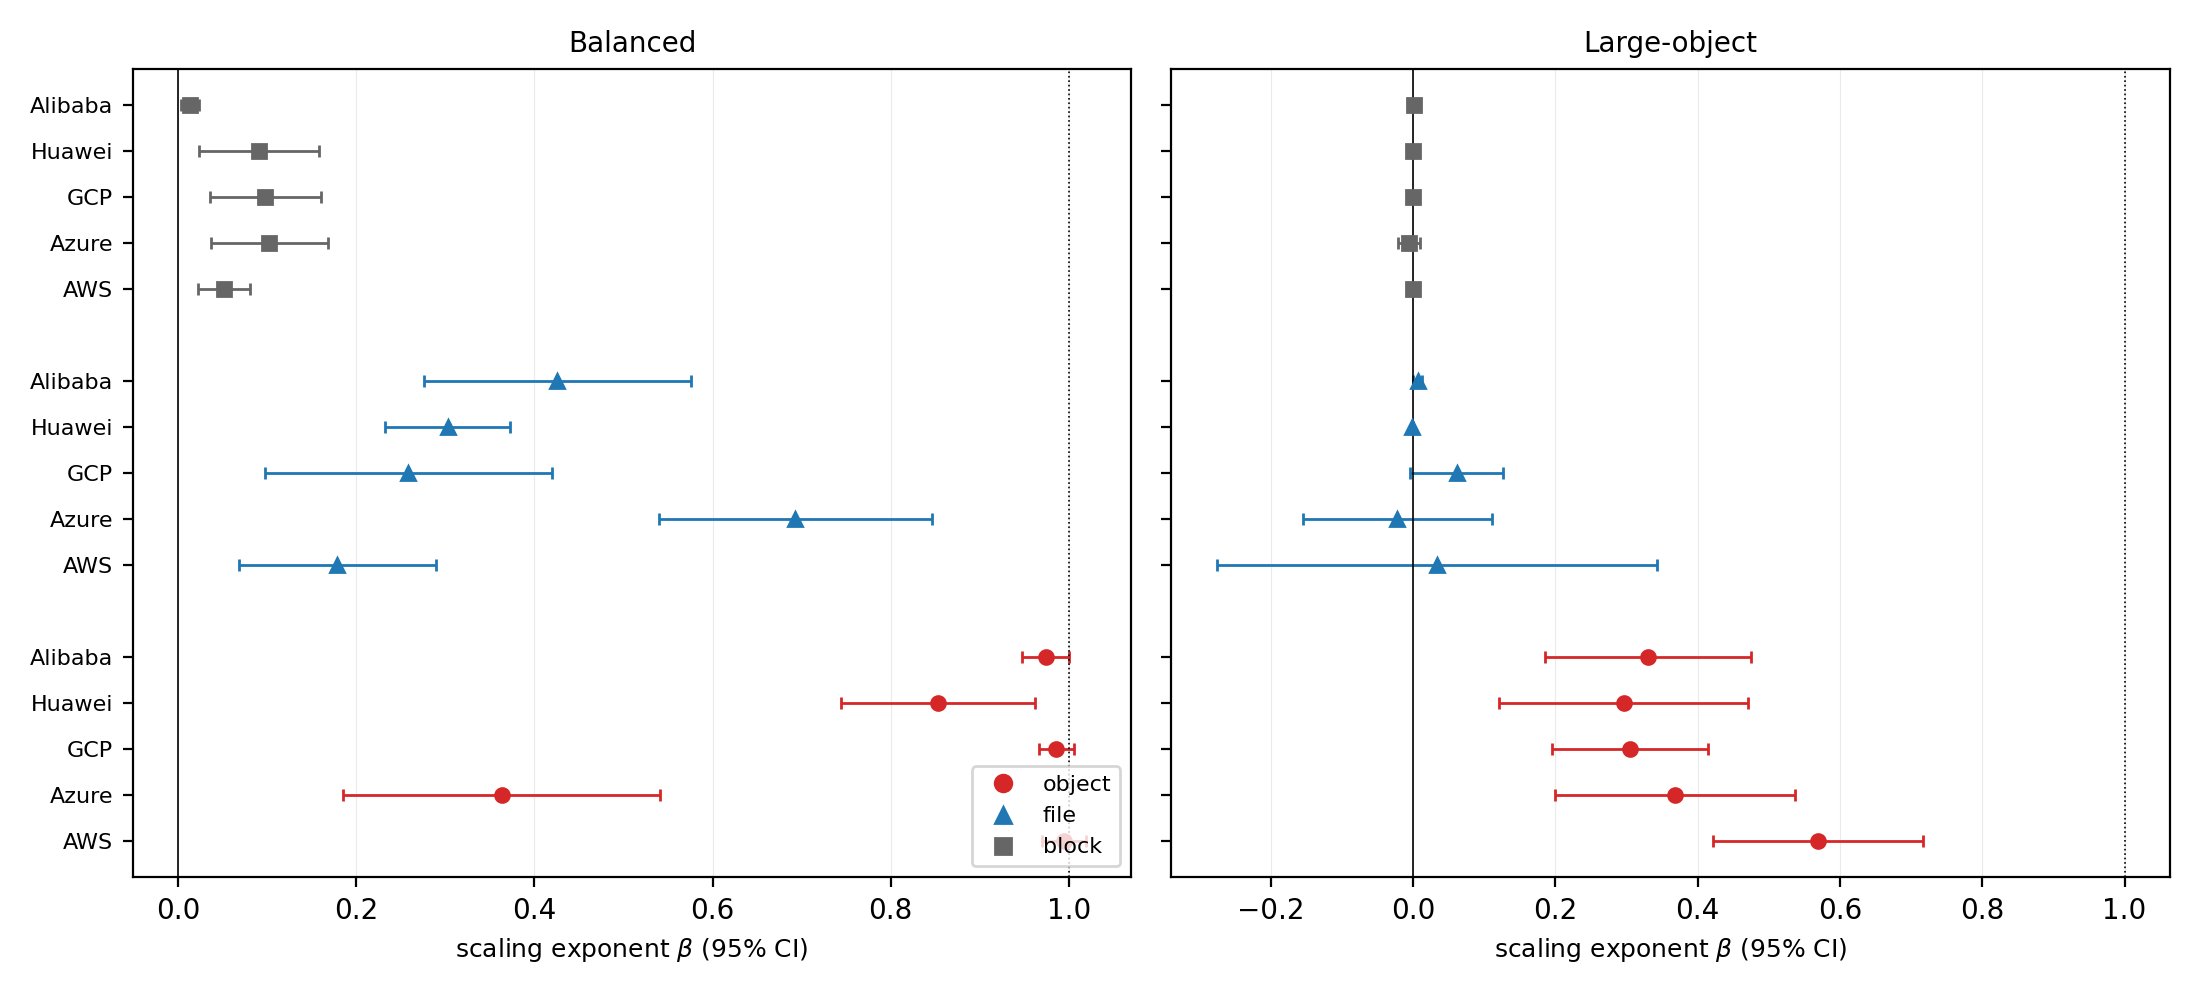
\includegraphics[width=0.9\textwidth]{figures/fig2_recomputed}
  \caption{Combined-throughput scaling exponents with 95\% confidence
  intervals. Reference lines at $\beta = 0$ and $\beta = 1$.}
  \Description{Two dot-and-error-bar panels showing scaling exponents per
  provider grouped by paradigm. Object exponents cluster near one in the
  balanced panel except Azure; block exponents cluster near zero in both
  panels; file exponents fall between zero and 0.7.}
  \label{fig:exponents}
\end{figure*}

Table~\ref{tab:exponents} and Figure~\ref{fig:exponents} report the
combined-rate fits; per-operation fits (write-phase and read-phase
separately) are in Appendix~A and lead to the same reading. Three regularities
organise the results. First, object-balanced exponents are 0.995 (AWS), 0.986
(GCP), 0.974 (Alibaba) and 0.853 (Huawei), each with $R^2 \geq 0.97$; Azure
Blob's is 0.363 with saturation at 16 threads, measured on the corrected
runner, and we report it as this account's measured service response rather
than generalising it to the platform. Second, block combined exponents lie
between $-0.01$ and 0.10 on four clouds in both classes; the Azure block
balanced cell fits 0.102 over the eight runs (three concurrency levels) that
completed both phases, with its four write-only runs contributing to the
write-phase fit only (Appendix~A). Third, file balanced exponents span
0.18--0.69 (Azure Files highest), while file large-object is at or below
0.06 everywhere.

Client-CPU sensitivity: excluding the 71 gated runs raises several object
exponents (e.g., AWS object large-object from 0.57 to 0.85) and materially
changes no block or file conclusion, indicating the 4 vCPU client
underestimated, rather than manufactured, object-storage scaling.

\subsection{Tail Latency by Phase}
\begin{figure*}
  \centering
  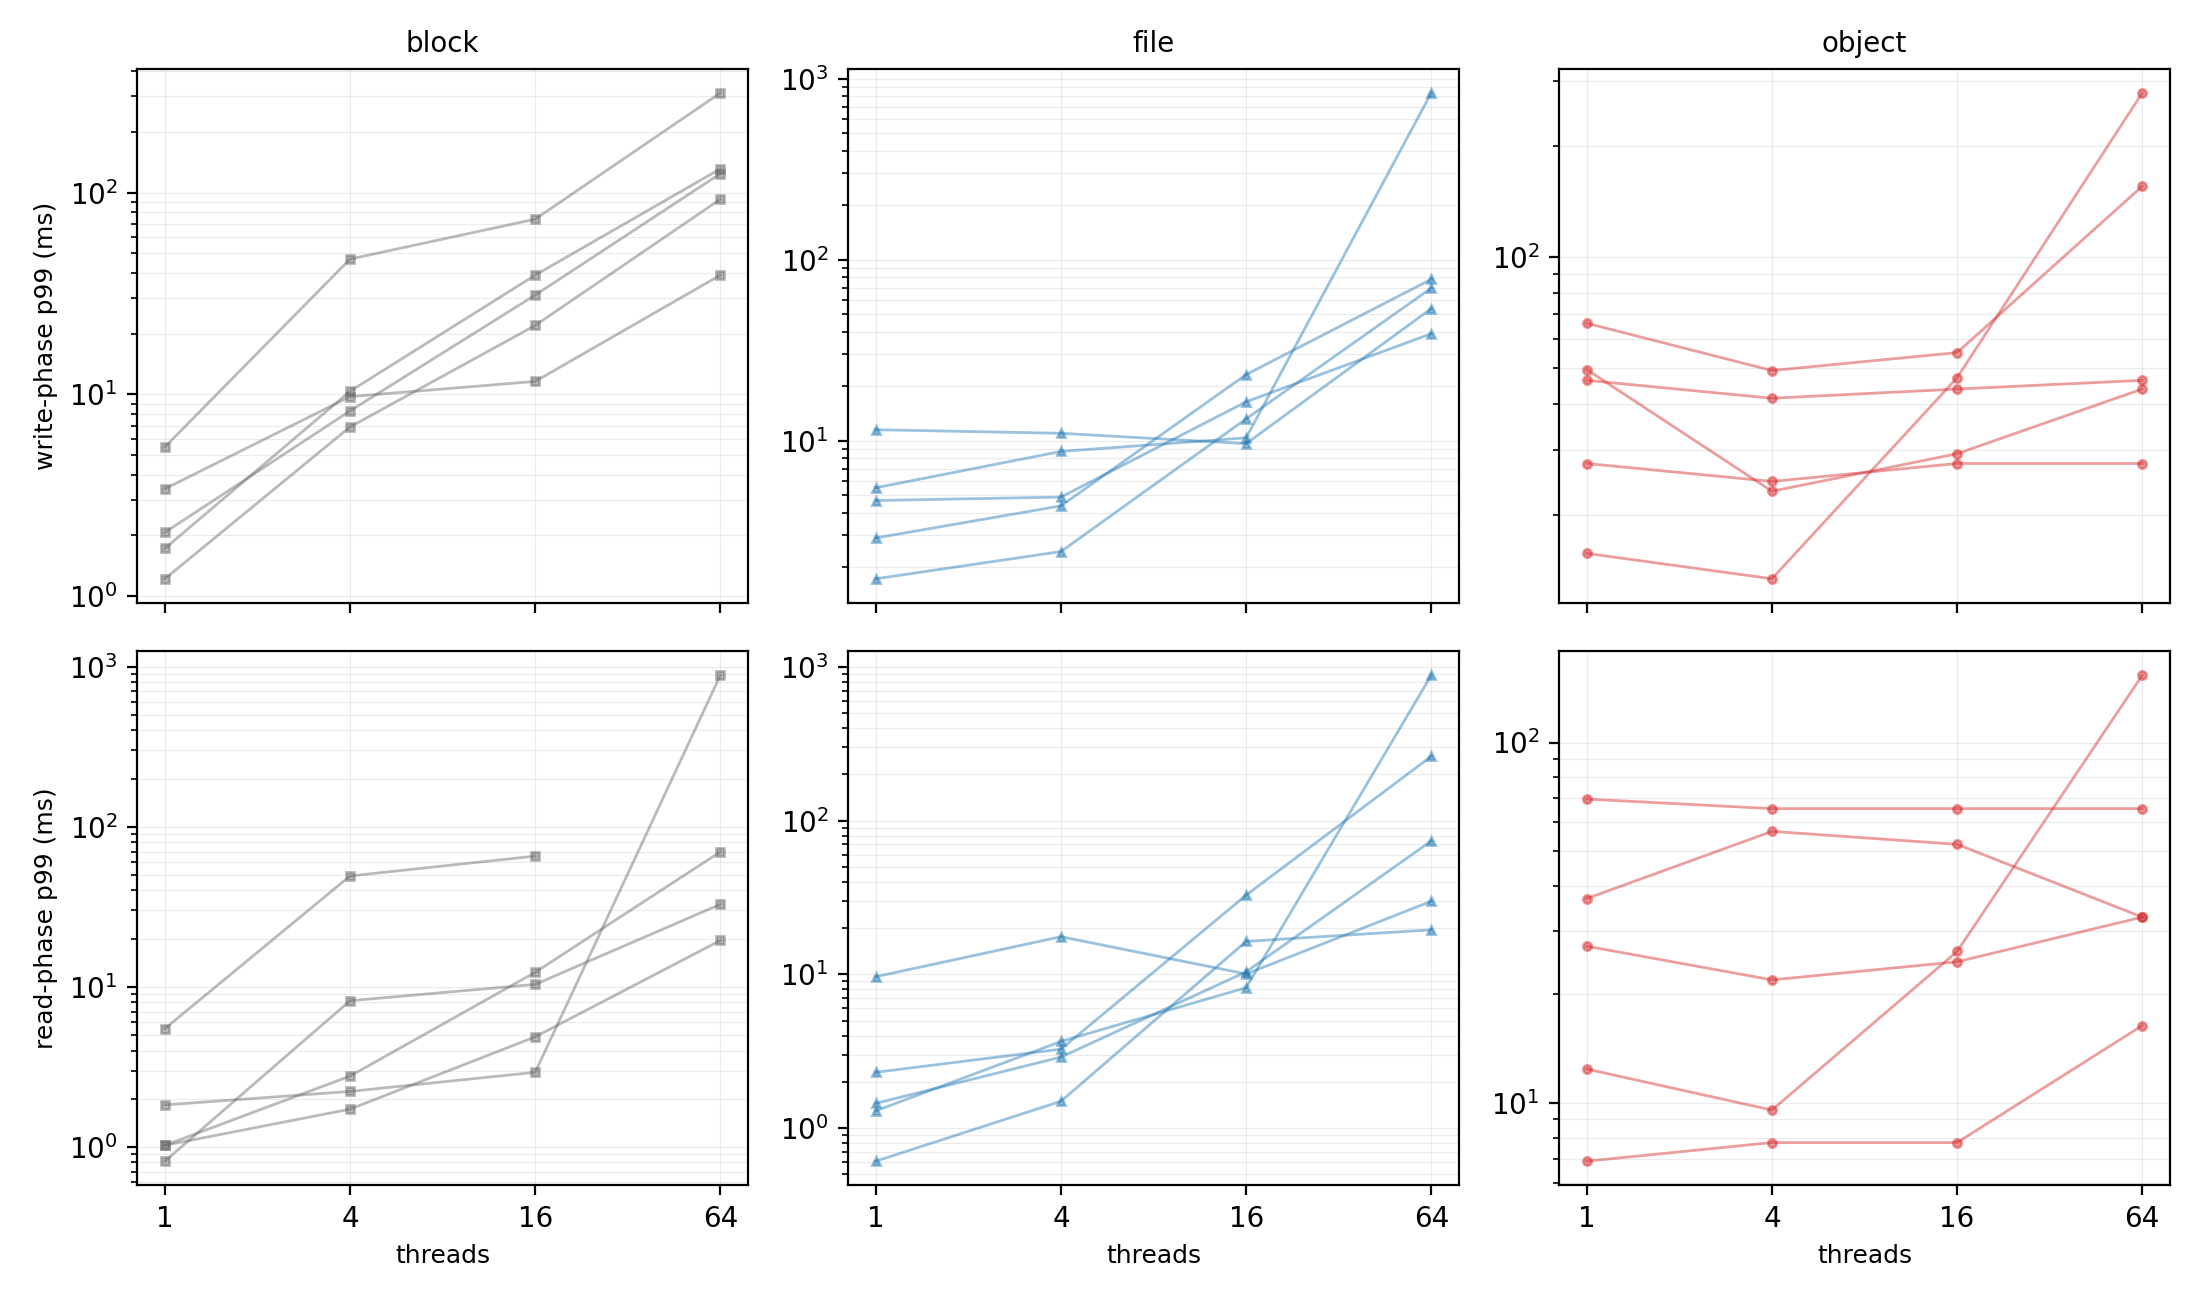
\includegraphics[width=0.95\textwidth]{figures/fig4_recomputed_p99}
  \caption{Per-phase p99 latency (balanced class), one line per provider.
  Write phases (top) and read phases (bottom) are never combined.}
  \Description{Six log-log panels of ninety-ninth percentile latency against
  thread count: write and read phases for block, file and object storage.
  Block and file latency lines climb steeply with thread count; object
  storage lines remain nearly flat.}
  \label{fig:latency}
\end{figure*}

From 1 to 64 threads in the balanced class, median write-phase p99 across
providers grows \pFoldWriteBlock-fold on block, \pFoldWriteFile-fold on file, and \pFoldWriteObject-fold on object
storage; read-phase medians grow \pFoldReadBlock-fold, \pFoldReadFile-fold and \pFoldReadObject-fold respectively
(Figure~\ref{fig:latency}). Where throughput does not scale, offered
concurrency appears as queueing delay; where it scales, tails hold. This is
the expected queueing behaviour of a capacity-bounded resource, observed here
per phase with no cross-phase aggregation.

\subsection{Provider Dependence of Slopes}
The mixed model (fixed effects: log concurrency $\times$ paradigm $\times$
workload; random provider intercept) is fitted over the $N = 356$ runs with
a defined combined rate. Adding a random provider slope gives a likelihood
ratio of 0.44: $p = 0.65$ against the boundary-corrected 50:50
$\chi^2_1$:$\chi^2_2$ mixture and $p = 0.55$ by parametric bootstrap. Both
the observed statistic and every bootstrap draw are fitted under an
explicit validity policy: each model is fitted with an optimizer ladder
(default, lbfgs, Powell) and represented by its highest \emph{finite}
converged log-likelihood; a draw is valid only if both models produce one
and the nested ordering $\ell_{\mathrm{alt}} \geq \ell_{\mathrm{null}}$
holds, so likelihood-ratio statistics are finite and non-negative by
construction rather than by clamping. Draws failing the policy are
rejected with recorded reasons, never counted. The archive holds 204
attempts yielding exactly 200 valid draws (batch seeds 42--46,
fixed-effects null baseline), each with its likelihoods, per-model
optimizers and warning counts (\texttt{boot\_draws.csv}). Mixed-model
optimisation at five groups is optimizer- and environment-sensitive:
draw-file byte-reproducibility is guaranteed only in the pinned container
published with the archive, and outside it agreement is statistical rather
than bytewise -- a limitation we state rather than hide, noting that all
three reference distributions agree the statistic is unremarkable under
the null. Two further honesty notes: estimating a slope variance from
five groups sits at the edge of what mixed models support, and earlier
drafts of this work reported successively LR $= 0.077$ (defective input:
four write-only runs in the combined rate) and a bootstrap without
finite-likelihood checks; both defects and their corrections are covered
by the archived regression tests.
Within this five-provider sample there is no evidence that scaling slopes
vary by provider once paradigm and workload are accounted for, while
provider effects on absolute level remain large. We state this as a
within-sample observation: five groups cannot rule out moderate slope
heterogeneity, and the one visible outlier (Azure object) is a single cell
that the variance component cannot represent.

\subsection{Consistency With the Fixed-Concurrency Dataset}
The sweep's 16-thread cells remeasure our earlier campaign's cells
\cite{thesis} on the same host class and regions. Using the earlier
campaign's own metric definitions for comparability, \consCellsWithin{} of \consCellsTotal{} cells agree
within ordinary cloud measurement variance (geometric-mean ratio \consGeoMean); the
two exceptions are the Azure object cells at 6.99$\times$ and 2.86$\times$,
which quantify the corrected runner defect rather than service drift. An
erratum note for the earlier report has been prepared accordingly.

\section{Discussion}
Read as provisioning guidance, the exponents say: parallelisable
small-operation traffic can be scaled against object storage on four of the
five measured clouds with near-unit efficiency until the client itself
saturates; entry-tier block volumes deliver their tier envelope regardless of
client thread count, with tail latency inflating by up to two orders of
magnitude under the added load; file services fall in between, with
meaningful provider differences in the balanced class.

We are careful about mechanism attribution. The flat block exponents are
\emph{consistent with} documented tier throughput caps (Table~\ref{tab:config}),
the flat file streaming results are \emph{consistent with} single-connection
protocol behaviour, and the large-object object-storage saturation at 16
threads is \emph{consistent with} the hosts' documented network limits -- but
neither the network path nor the protocol layer was instrumented directly,
so these attributions remain hypotheses supported by configuration records
rather than demonstrated causes; per-paradigm causal isolation (premium-tier
contrasts, protocol tracing) is future work under the replication protocol.

The null result on provider slopes, combined with the earlier campaign's
strong provider effects on absolute performance, suggests a practical
heuristic within the bounds of this design: paradigm choice determines how
performance grows with parallelism, provider choice determines the level at
which it starts. The heuristic's scope is one host class, one region per
provider, entry tiers and two workload classes.

\section{Threats to Validity}
\emph{Construct.} Two phase-pure data-movement classes probe a narrow slice
of storage behaviour; metadata-intensive and interleaved mixed workloads are
excluded by design. The combined rate is defined only for runs with both
phases and is secondary to per-operation rates. \emph{Internal.} Executed
conditions vary as quantified in Section~\ref{sec:asexecuted}; steady-state
per-operation rates are the analysis quantities precisely because they are
robust to those variations, and the full condition record ships with the
dataset. The client is a single 4 vCPU host per provider; 71 runs crossed
the CPU gate, and sensitivity refits move object exponents upward only.
Instrument corrections were handled by quarantine and remeasurement, with
defective data preserved. Per-run instrument hashes were not recorded (a v1
reporting gap fixed in the replication protocol). \emph{External.} One
region per provider, entry tiers, single accounts, a 2026 snapshot. The
provider-slope null is bounded by five groups. \emph{Statistical.} No
analysis choice was independently registered before data collection; all
inferential statements should be read as exploratory.

\section{Conclusion}
Across 360 accepted runs on five public clouds, object storage was the only
managed paradigm whose small-operation throughput scaled with client
concurrency (exponents 0.85--1.00 on four clouds, with one measured
exception), block storage at entry tiers showed no useful scaling while its
p99 latency grew by up to two orders of magnitude, and file storage sat in
between. Scaling slopes aligned with paradigm architecture; provider identity
moved absolute levels but showed no detectable effect on slopes within this
sample. The complete evidence chain -- raw artefacts, every attempt,
telemetry, quarantined defective-instrument data, the recomputation pipeline
and a locked replication protocol -- is public, and we offer the two
instrument failure modes documented here as cautionary results in their own
right.

\begin{acks}
This work extends the first author's MTech research at the Cape Peninsula
University of Technology. Cloud consumption was funded by the authors'
research allocation; no provider had any role in design, execution or
reporting.
\end{acks}

\section*{Data Availability}
Dataset, harness, Terraform definitions, recomputation and figure pipelines,
regression tests, as-executed configuration record, quarantined data, the
manuscript source itself and the locked replication protocol:
\url{https://github.com/tshivhidzo/cloud-storage-bench}, annotated tag
\texttt{sweep-v1-audited-r8}. Immutable audited version DOI:
\texttt{10.5281/zenodo.22058064}; all-versions concept DOI:
\url{https://doi.org/10.5281/zenodo.22032835}. Superseded tags r1--r7 are
preserved, including publication attempts retained for audit-trail
completeness (r5: 10.5281/zenodo.22056327; r6: 10.5281/zenodo.22057377;
r7: 10.5281/zenodo.22057803, whose deposit and tag diverged). A pinned
reproduction container (Dockerfile + full dependency lock) is included;
bootstrap draw-file byte-identity is guaranteed inside it. Code MIT; data
CC BY 4.0.

\appendix
\section{Per-Operation Exponents}
\begin{table}[h]
\caption{Write-phase and read-phase scaling exponents per cell, generated
directly from the archived analysis output.}
\small
\begin{tabular}{llllrlrr}
\toprule
Provider & Paradigm & Workload & Op & $\beta$ & 95\% CI & $R^2$ & $N$ \\
\midrule
Alibaba & block & balanced & write & -0.001 & $[-0.003, 0.001]$ & 0.205 & 12 \\
Alibaba & block & balanced & read & 0.028 & $[0.009, 0.047]$ & 0.512 & 12 \\
Alibaba & block & large-object & read & 0.002 & $[0.001, 0.002]$ & 0.659 & 12 \\
Alibaba & file & balanced & write & 0.478 & $[0.324, 0.631]$ & 0.828 & 12 \\
Alibaba & file & balanced & read & 0.363 & $[0.217, 0.508]$ & 0.756 & 12 \\
Alibaba & file & large-object & read & 0.007 & $[0.001, 0.013]$ & 0.372 & 12 \\
Alibaba & object & balanced & write & 0.977 & $[0.963, 0.992]$ & 1.0 & 12 \\
Alibaba & object & balanced & read & 0.966 & $[0.9, 1.033]$ & 0.991 & 12 \\
Alibaba & object & large-object & read & 0.33 & $[0.186, 0.474]$ & 0.723 & 12 \\
AWS & block & balanced & write & 0.029 & $[0.013, 0.046]$ & 0.61 & 12 \\
AWS & block & balanced & read & 0.098 & $[0.042, 0.155]$ & 0.6 & 12 \\
AWS & block & large-object & read & -0.0 & $[-0.001, 0.001]$ & 0.007 & 12 \\
AWS & file & balanced & write & 0.225 & $[0.096, 0.354]$ & 0.6 & 12 \\
AWS & file & balanced & read & 0.118 & $[-0.012, 0.248]$ & 0.292 & 12 \\
AWS & file & large-object & read & 0.034 & $[-0.276, 0.343]$ & 0.006 & 12 \\
AWS & object & balanced & write & 0.986 & $[0.972, 1.0]$ & 1.0 & 12 \\
AWS & object & balanced & read & 1.004 & $[0.948, 1.059]$ & 0.994 & 12 \\
AWS & object & large-object & read & 0.569 & $[0.422, 0.716]$ & 0.881 & 12 \\
Azure & block & balanced & write & -0.011 & $[-0.043, 0.02]$ & 0.06 & 12 \\
Azure & block & balanced & read & 0.163 & $[0.072, 0.255]$ & 0.76 & 8 \\
Azure & block & large-object & read & -0.006 & $[-0.022, 0.009]$ & 0.073 & 12 \\
Azure & file & balanced & write & 0.686 & $[0.506, 0.866]$ & 0.878 & 12 \\
Azure & file & balanced & read & 0.697 & $[0.555, 0.838]$ & 0.923 & 12 \\
Azure & file & large-object & read & -0.022 & $[-0.155, 0.111]$ & 0.014 & 12 \\
Azure & object & balanced & write & 0.31 & $[0.131, 0.488]$ & 0.599 & 12 \\
Azure & object & balanced & read & 0.401 & $[0.222, 0.579]$ & 0.714 & 12 \\
Azure & object & large-object & read & 0.368 & $[0.2, 0.536]$ & 0.704 & 12 \\
GCP & block & balanced & write & 0.055 & $[0.013, 0.097]$ & 0.458 & 12 \\
GCP & block & balanced & read & 0.173 & $[0.074, 0.273]$ & 0.6 & 12 \\
GCP & block & large-object & read & 0.0 & $[0.0, 0.0]$ & 0.53 & 12 \\
GCP & file & balanced & write & 0.245 & $[0.077, 0.412]$ & 0.515 & 12 \\
GCP & file & balanced & read & 0.365 & $[0.248, 0.482]$ & 0.828 & 12 \\
GCP & file & large-object & read & 0.061 & $[-0.004, 0.127]$ & 0.302 & 12 \\
GCP & object & balanced & write & 0.948 & $[0.924, 0.973]$ & 0.999 & 12 \\
GCP & object & balanced & read & 1.03 & $[1.006, 1.054]$ & 0.999 & 12 \\
GCP & object & large-object & read & 0.305 & $[0.195, 0.414]$ & 0.794 & 12 \\
Huawei & block & balanced & write & 0.003 & $[-0.043, 0.049]$ & 0.002 & 12 \\
Huawei & block & balanced & read & 0.281 & $[0.126, 0.435]$ & 0.621 & 12 \\
Huawei & block & large-object & read & 0.0 & $[-0.001, 0.001]$ & 0.001 & 12 \\
Huawei & file & balanced & write & 0.432 & $[0.343, 0.521]$ & 0.921 & 12 \\
Huawei & file & balanced & read & 0.034 & $[0.012, 0.057]$ & 0.537 & 12 \\
Huawei & file & large-object & read & -0.001 & $[-0.001, -0.001]$ & 0.725 & 12 \\
Huawei & object & balanced & write & 0.848 & $[0.713, 0.982]$ & 0.952 & 12 \\
Huawei & object & balanced & read & 0.86 & $[0.786, 0.933]$ & 0.986 & 12 \\
Huawei & object & large-object & read & 0.296 & $[0.121, 0.471]$ & 0.587 & 12 \\
\bottomrule
\end{tabular}

\end{table}

\bibliographystyle{ACM-Reference-Format}
\bibliography{refs2}

\end{document}
